\section{Unified Virtual Layer}
To realize unified RDMA virtualization for containers and virtual machines,  we propose a software RDMA virtualization framework, namely uniRDMA. The vRNIC constructed by uniRDMA based on the user space virtualization layer provides unified virtual RDMA for virtual machines or containers.

As Figure~\ref{fig:framework-overview} shows, uniRDMA is consist of two parts: uniRDMA user space virtual layer and uniVerbs interface. The former is responsible for the establishment and management of virtual RDMA. The specific work includes the virtualization of vRNIC, the mapping management of vRNIC to VF, and the virtual RDMA network management, such as virtual RDMA address configuration and routing; the latter is mainly aout how RDMA applications use vRNICs, including the construction of general interfaces and the optimization.

\begin{figure}[!ht]
	\centering
	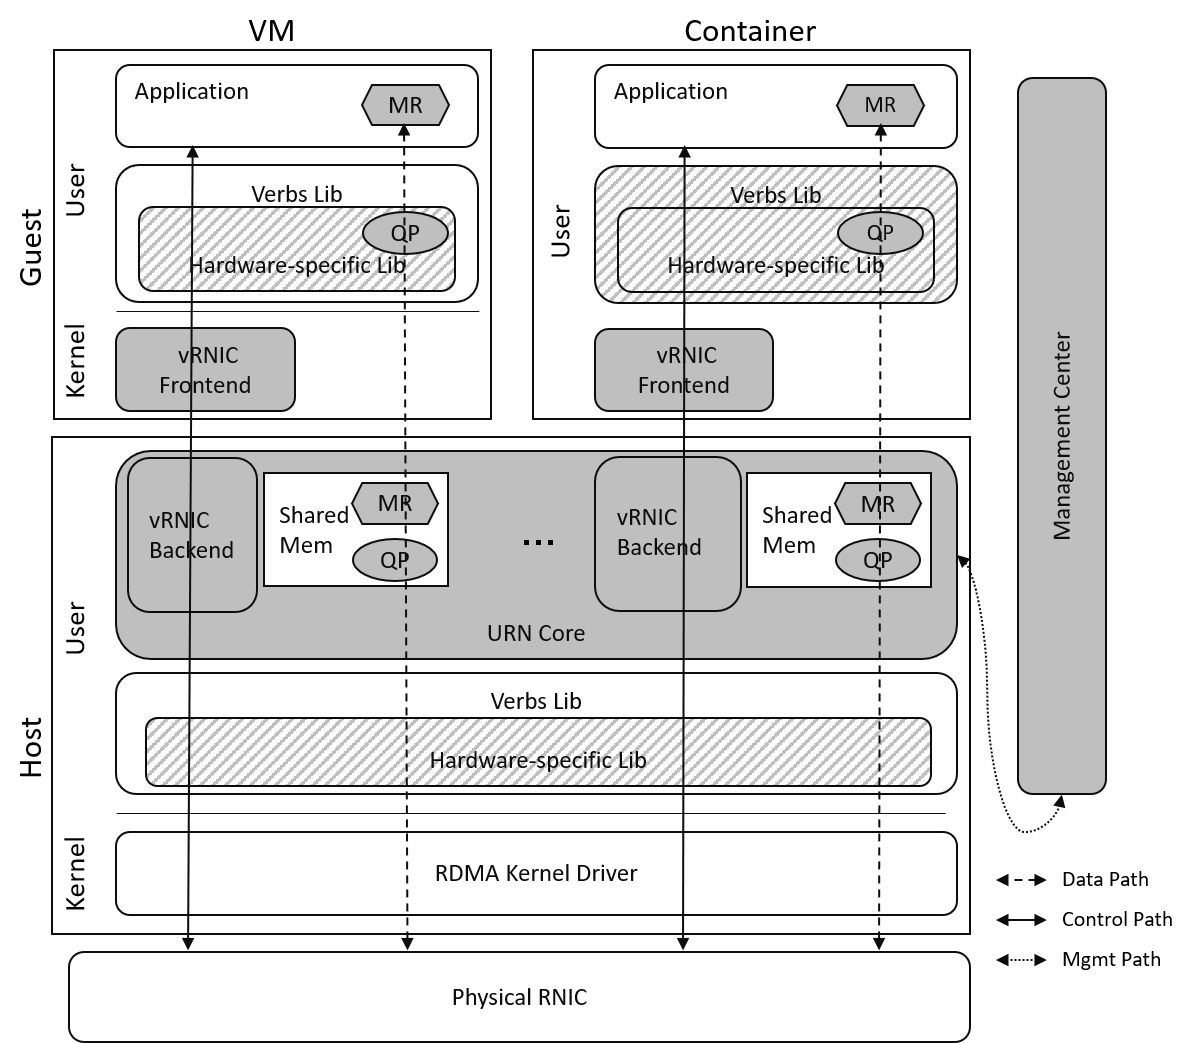
\includegraphics[width=1.0\linewidth]{images/framework-overview}
	\caption{uniRDMA Framwork Overview}
	\label{fig:framework-overview}
\end{figure}
